 
%\documentclass[10pt, conference, compsocconf]{IEEEtran}
\documentclass[twocolumn]{svjour3}


% *** CITATION PACKAGES ***
\usepackage{amsmath}
\usepackage{fullpage}
\usepackage[utf8]{inputenc}
\usepackage{mathtools}
\usepackage{amssymb}
\usepackage{graphicx}
\usepackage{caption}
\usepackage{subcaption}
%\usepackage{amsthm}
\usepackage{aliascnt}

\usepackage{algpseudocode}
\usepackage{algorithm} 


\DeclarePairedDelimiter{\ceil}{\lceil}{\rceil}

\usepackage[usenames,dvipsnames]{color}
%\usepackage[colorlinks=true,urlcolor=OliveGreen,citecolor=Blue]{hyperref}

\usepackage{soul}
\usepackage{xspace}
\usepackage{hyperref} 

%\newtheorem{theorem}{Theorem}
%\newtheorem{corollary}{Corollary}[theorem]
%\newtheorem{lemma}[theorem]{Lemma}

\newcommand{\todo}[1]{{\color{red}\textbf{\hl{#1}}\xspace}}

%\graphicspath{{C:\Users\Manmohan\Documents\GitHub\research}}

% *** GRAPHICS RELATED PACKAGES ***
% 
%\ifCLASSINFOpdf
  % \usepackage[pdftex]{graphicx}
  % declare the path(s) where your graphic files are
  % \graphicspath{{../pdf/}{../jpeg/}}
  % and their extensions so you won't have to specify these with
  % every instance of \includegraphics
  % \DeclareGraphicsExtensions{.pdf,.jpeg,.png}
%\else
 
%\fi

% correct bad hyphenation here
\hyphenation{op-tical net-works semi-conduc-tor}


\makeatletter
\renewcommand*{\thetable}{\arabic{table}}
\renewcommand*{\thefigure}{\arabic{figure}}
\let\c@algocf\@undefined
\newaliascnt{algocf}{figure}
\let\c@table\@undefined
\newaliascnt{table}{figure}
\let\c@table\c@figure

\makeatother

\begin{document}

\title{Replicated Data Placement for Uncertain Scheduling}

\author{Manmohan Chaubey \and Erik Saule}

\institute{E. Saule \at Department of Computer Science\\
 University of North Carolina at Charlotte\\
 Charlotte, USA\\
Tel: +1 (704) 687-8580 \\
\email{esaule@uncc.edu}}

% \author{\IEEEauthorblockN{Manmohan Chaubey and Erik Saule }
% \IEEEauthorblockA{Department of Computer Science\\
%  University of North Carolina at Charlotte\\
%  Charlotte, USA\\
%  Email: mchaubey@uncc.edu, esaule@uncc.edu}
% }

\maketitle


\begin{abstract}
\todo{rewrite}

  Scheduling theory is a common tool to analyze the performance of
  parallel and distributed computing systems, such as their load
  balance. How to distribute the input data to be able to execute a
  set of tasks in a minimum amount of time can be modeled as a
  scheduling problem. Often these models assume that the computation
  time required for each task is known accurately. However in many
  practical case, only approximate values are available at the time of
  scheduling.

  In this paper, we investigate how replicating the data required by
  the tasks can help coping with the inaccuracies of the processing
  times. In particular, we investigate the problem of scheduling
  independent tasks to optimize the makespan on a parallel system
  where the processing times of the tasks are only known up to a
  multiplicative factor. The problem is decomposed in two phases: a
  first offline phase where the data of the tasks are placed and a
  second online phase where the tasks are actually scheduled.

  For this problem we investigate three different strategies, each
  allowing a different degree of replication of tasks: a) No
  Replication b) Replication everywhere and c) Replication in
  groups. We propose approximation algorithms and theoretical lower
  bound on achievable approximation ratios.  This allows us to study
  the tradeoff between the number of replication and the guarantee on
  the makespan.

  \keywords{Scheduling \and Uncertainty \and Robustness \and
    Replication \and Approximation Algorithms \and Parallel System}
\end{abstract}


\section{Introduction}

Parallel and distributed computing systems are often modeled using
tasks that are processed simultaneously on different
machines. Studying the balance of the load of the various component of
the system is often key in understanding the performance one obtains
in practice. A system typically schedules the set of tasks with the
goal of optimizing the load balance (or makespan) of the system or
some other metric. A key information these systems use to plan the
execution is the time tasks will take to be processed. However, this
information is typically not precisely known in practice: because the
user can only make a wild guess on the runtime of her
task~\cite{Luong2008}, because prediction is hard in the general
case~\cite{Wilhelm2008}, or because underlying models of a particular
algorithm can only predict runtime within a given
range~\cite{Erlebacher14-ICS}. Whichever the reason is, not knowing
accurately the processing time can significantly impact the
performance obtained from the machine.

Though, the uncertainty of processing times is only a real problem if
the tasks are pinned to particular computing units. If a task could
be moved as the system sees fit without incurring an extra cost, the
problem would be vastly alleviated. The problem is that, in practice,
a task has to run on a particular machine because the input data for
this task are only available on this machine. This is the case in most
parallel and distributed systems and it is particularly true in
out-of-core computing systems. For instance in out-of-core sparse
linear algebra, executing a task where the data are not locally
available would have a prohibitive
overhead~\cite{Zhou12-Cluster,Zhou12-P2S2}.

One approach for dealing with the uncertainty of processing times is
to build a robust
schedule~\cite{cj09c,Gatto07,Davenport_slack-basedtechniques}, that
is, building a schedule that can naturally cope with variations in the
processing times. These techniques often use sensitivity analysis to
determine the robustness of the schedule. However, a better approach
would be to be able to dynamically change the schedule.

The idea we are pursuing in this paper is to replicate the input data
of the tasks onto multiple machines. This way, when the actual
processing times of the tasks are too different from their
estimations, the system will have some room to adapt at runtime. This
is certainly feasible in practice as many system have more memory than
the computation use. For instance, most Hadoop system replicates the
data for the purpose of tolerating hardware
faults~\cite{White:2009:HDG:1717298}. And it has been shown that
launching the same task multiple times can help cope with hardware
differences~\cite{DBLP:journals/corr/WangJW14} but increases resource
usage. The cost of replicating the data might be amortized in many
applications where the application will iterate over the data multiple
times ({\em e.g.}, in an iterative
solver~\cite{Zhou12-P2S2,Zhou12-Cluster}). In this paper, we answer
the question ``can data replication help cope with the uncertainty of
processing time?'' by considering two different models of the cost of
replicating tasks. Under either model, we show that replication does
help dealing with uncertainty.

In the first case, we model the cost of replication simply by allowing
a given number of replica for each task: we will propose a lower bound
when no replication is allowed and propose algorithms for the three
cases where no replication is allowed, the tasks are replicated
everywhere and the number of replica is bounded by an integer
$k$. We introduced this model in~\cite{Chaubey2015}.

In the second model, we measure the per processor cost of the tasks
that are replicated on it. In a computer system context, placing a
task on a processor increases the required memory of this
processor. Rather than bounding the available memory, we treat the
maximum memory occupation as a objective to minimize in itself. Memory
occupation boils down to a secondary makespan objective (except it
does not suffer from uncertainty). We investigated the memory-makespan
tradeoff in the case of certain processing times (and no replication)
in~\cite{SDM2008}. We analyze the non-replication algorithm
of~\cite{SDM2008} under the uncertain processing time model. And we
propose a new memory-aware replication algorithm that provides more
interesting memory makespan tradeoffs.

The remaining of the paper is organized as follows: we describe system
model and notations in Section~\ref{sec2}. Related works are presented
in Section~\ref{sec3}.  Section~\ref{sec4} investigates what can be
done if the tasks can only be deployed on a single machine, we
provide a guaranteed algorithm and provide a lower bound on the best
guarantee that one can achieve in this case. Section~\ref{sec5} takes
the reverse case and investigates what can be achieved if the data are
replicated everywhere, leaving the maximum flexibility at runtime. We
investigate one algorithm in this case and analyze its performance
guarantee. Section~\ref{sec6} investigates grouping machines
together and replicating data in these groups as an intermediate
between the previous two strategies and provide a guaranteed algorithm
in that case. Section~\ref{sec7} summarizes the various results we
derived and study the tradeoff between performance guarantee and data
replication.


\section{Related Work}\label{sec3}

When no replication is allowed, the problem is exactly the classical
independent tasks scheduling problem on identical machines, which is
known to be NP-Hard~\cite{GareyJohnson79}. We use Graham's List
Scheduling (LS)~\cite{Graham66} and Largest Processing Time (LPT)
algorithms~\cite{Graham69boundson} to derive approximation ratios in
different scenarios. The LS algorithm takes tasks one at a time and
assigns them to the machine having the least load at that time. LS is
a 2-approximation algorithm and is widely used in online scheduling
problems. LPT sorts the tasks in a non-increasing order of processing
time and assigns them one at a time in this order to the machine with
the smallest current load. The LPT algorithm has a worst case
approximation ratio of $\frac{4}{3}$ in the offline
setting. One can even obtain an arbitrarily good approximation
algorithm for this problem by increasing its complexity with a dual
approximation algorithm~\cite{Hoch87}.


Based on various models for describing the uncertain input parameters,
various methodologies can be used including reactive, stochastic,
fuzzy and robust approach~\cite{DBLP:journals/cce/LiI08}. We are using
the bounded uncertainty model which assumes that an input parameter
has a value between a lower and upper bound.  Wierman and
Nuyens~\cite{conf/sigmetrics/WiermanN08} introduce SMART, a
classification to understand size-based policies and draw analytic
co-relation between response time and estimated job size in single
server problem. Robust approaches to deal with uncertainty are widely
used on MapReduce
systems~\cite{Kavulya:2010:ATP:1844765.1845224,Verma:2011:AAR:1998582.1998637},
in
Hadoop~\cite{Wolf:2010:FSA:2023718.2023720,White:2009:HDG:1717298},
on databases~\cite{Lipton199518} and on web
servers~\cite{Cardellini99dynamicload}. The HSFS and FLEX schedulers
provide robustness in scheduling against uncertain job
size~\cite{Wolf:2010:FSA:2023718.2023720,6691554}. Cannon and
Jeannot~\cite{cj09c} analyzed the correlation between various metrics
used to measure robustness and provided scheduling heuristics that
optimizes both makespan and robustness for scheduling task graph on
heterogeneous system.

Most of the work on robust scheduling use scenarios to structure
the variability of uncertain parameters. Daniels and
Kouvelis~\cite{citeulike:8334169} used them to optimize the flow-time
using a single machine. Davenport, Gefflot, and Bek analyzed slack
based technique (adding extra idle time) to cope with
uncertainty~\cite{Davenport_slack-basedtechniques}. Gatto and Widmayer
derive bounds on competitive ratio of Graham’s online algorithm in
scenarios where the processing times of tasks either increase or decrease
arbitrarily due to perturbations~\cite{Gatto07}.  These works
considered augmenting or decreasing of job processing times as
different problem scenarios that need to be optimized. We 
approach the problem using worst case analysis where some tasks may
increase and some may decrease within the same schedule.
  
Data placement and replication methodologies are highly used in
distributed systems including peer-to-peer and Grid systems to achieve
effective data management and improve
performance~\cite{Cirne2007213,Abawajy,4215379}. Tse~\cite{DBLP:journals/tc/Tse12}
used selective replication of documents to increase the available
bandwidth to serve files using web servers and study the problem
through bi-criteria optimization techniques to maximize the quality of
service and minimize the memory occupation.


\section{Problems Definition}\label{sec2}
Let $J$ be a set of $n$ tasks which need to be scheduled onto a set
$M$ of $m$ machines. Notice that scheduling theory commonly use
interchangeably the terms ``machines'' and ``processors'' and the
terms ``jobs'' and ``tasks''. We are considering the problem where the
scheduler does not know the processing time $p_j$ of task $j$
precisely before the task completes.  But the scheduler has access to
some estimation of the processing time $\tilde{p_j}$ of task $j$
before making any scheduling decisions. We assume that the actual
processing time $p_j$ of a task $j$ is within a multiplicative factor
$\alpha$ of the estimated processing time $\tilde{p_j}$. (An
inaccuracy of the throughput of the system leads to a multiplicative
error and any interval of confidence of a runtime can be transformed
into a value and a multiplicative error.) $\alpha$ is a quantity known
to the scheduler. In other words the scheduler knows that:
 \begin{equation}\label{eq1}
\frac{\tilde{p}_{j}}{\alpha}\leq p_{j}\leq \alpha \tilde{p}_{j}
\end{equation}

Assuming that the processing time of the tasks is known to be in an
interval is reasonable in many application scenarios. One could derive
bounds experimentally using machine learning techniques: for
instance~\cite{You14-ICPP} used Support Vector Machines to predict the
time it will take to run graph traversal algorithms. Models of runtime
of algorithms can also be derived analytically:
in~\cite{Erlebacher14-ICS} the authors provide bounds for the
performance of various sparse linear algebra operations using only the
size of the matrices and vectors involved.

Scheduling for this problem is performed in two phases. Phase 1
chooses where data are replicated using the estimated processing time
$\tilde p_j $, for each of the task $j$. The phase takes
$\tilde{p_j}$, $m$ and $\alpha$ as inputs and outputs sets of
machines, $M_j \subseteq M $ where each task $j$ can be
scheduled. This phase is purely offline and corresponds to the
operations performed to prepare the execution of the application.

Phase 2 takes the output of phase 1 as its input and maps each task
$j$ to a machine within the set of machines $M_j$. For each machine
$i$, let $E_i \subseteq J$ be the set of tasks assigned to machine
$i$. This phase chooses the actual schedule following an online
semi-clairvoyant process. Only the approximate processing time is
known when a task is placed, but the scheduler can wait for a machine
to become idle, to place the next one. Therefore, it can dynamically
schedule the tasks and the actual processing time of the tasks are
known once they complete.

The problem is to optimize the makespan, $C_{max} = \max_i \sum_{j \in
  E_i} p_j$ which is the completion time of the last task of the
system. $C_{max}^{*}$ denotes the optimal makespan of an instance of
the problem (knowing the actual processing times). An offline
algorithm is said to be a $\rho$-approximation algorithm (or to have
an approximation ratio of $\rho$) if it guarantees for all the
instances that $C_{max} \leq \rho C_{max}^*$. When the problem is
online, we are talking about competitive ratios. And we will use the
online language here since our problem is partly online.

In the {\bf the replication bound model}, the cost of replication is
modeled by using a task centric approach. Each task must be replicated
less than $k$ times, that is to say $\forall j, | M_j | \leq k$. In
this model, we will provide algorithms that take $k$ as a parameter. .

In {\bf the memory-aware model} each task $j$ has a size $s_j$. The
memory occupation $Mem_i$ of processor $i$ is the total size of the
task replicated on $i$: $Mem_i = \sum_{j \in E_i} s_j$. And the
problem is to minimize the maximum memory occupation $Mem_{max} =
\max_i Mem_i$. Notice that $Mem_{max}$ is an objective similar to the
makespan. In this model, we will provide bi-objective algorithm and
will measure their quality by using Zenith-approximation. That is to
say, we will design algorihtms to be competitive on the makespan and
approximated on the memory occupation at the same.


\section{The Replication Bound Model}

\subsection{Lower Bound}

\begin{theorem}
\label{th:model1-lb}
When $\forall j, |M_j| = 1$, there is no online algorithm having
competitive ratio better than $\frac{\alpha^{2}m }{\alpha^{2} + m-1}$.
\end{theorem}
 
\begin{proof}
  We use the adversary technique to prove the lower bound of this
  theorem. An adversary discloses the input instance piece by
  piece. It analyzes the choices made by the algorithm to change the
  part of the instance that has not been disclosed yet. That way it
  can build an instance that maximizes the competitive ratio of the
  algorithm.
 
  Let us consider an instance with $\lambda m$ tasks of equal
  estimated processing time $\forall j, \tilde{p_j} = 1$. After phase
  1, let $i$ be the most loaded machine which has $B$
  tasks. Obviously, $B \geq \lambda$. In phase 2 the adversary
  increases the processing time of the tasks on machine $i$ by a
  factor of $\alpha$ and changes the processing time of the other
  tasks by a factor of $\frac{1}{\alpha}$. So, $ C_{max}$ = $\alpha
  B$. ${C^{*}_{max}}$ will be no worse than any feasible solution. In
  particular, the solution that distributes equally the tasks of size
  $\alpha$ and the tasks of size $\frac{1}{\alpha}$. Therefore
  ${C^{*}_{max}} \leq \frac{1}{\alpha }\ceil {\frac{\lambda m - B
    }{m}}+ \alpha\ceil{\frac{B}{m}} $.  Figure~\ref{fig:rara} depicts
  the online solution and the offline optimal. We have,
 \begin{equation}\nonumber
   \frac{C_{max}}{C^{*}_{max}}
   \geq \frac{\alpha^{2} B  }{\ceil{\frac{
        \lambda m - B }{m}}+\alpha^2\ceil{\frac{B}{m}}}
 \end{equation}
   
 Since $\frac{ \lambda m - B }{m} +1 \geq\ceil{\frac{ \lambda m - B
   }{m}}$ and $\frac{B}{m}+1\geq\ceil{\frac{B}{m}}$, we have
 \begin{equation}\nonumber
   \frac{C_{max}}{C^{*}_{max}}
   \geq \frac{\alpha^{2} B  }{\frac{
       \lambda m - B }{m}+1+\alpha^2\frac{B}{m}+\alpha^{2}}
 \end{equation}
 
 From above expression it is clear that the smaller the value of $B$, the more the
 value of the expression decreases. So, any algorithm should minimize
 $B$ to achieve better performance.  For a schedule to be feasible the
 condition $B \geq \lambda$ must be satisfied. For $B = \lambda$ the
 value of $\frac{C_{max}}{C^{*}_{max}}$ is minimum and is equal to
 $\frac{\alpha^{2} m \lambda }{\lambda(\alpha^{2}+m-1)+
   m(\alpha^{2}+1)}$. The adversary can maximize the ratio of the
 algorithm by arbitrarily increasing $\lambda$. When $\lambda$ tends
 to $\infty$, we have
 \begin{equation}\nonumber
       \frac{C_{max}}{C^{*}_{max}}
       \geq \frac{\alpha^{2}m  }{\alpha^{2}+m-1}
     \end{equation}
 

  \begin{figure}[htp]
  \centering
  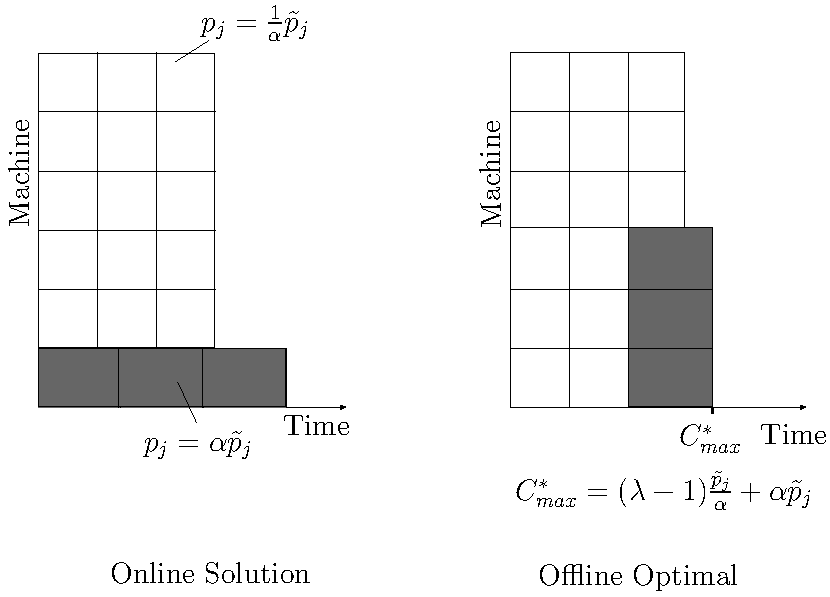
\includegraphics[width= 8 cm]{model1.pdf}
  \caption{Instance constructed by the adversary in the proof of
    theorem~\ref{th:model1-lb} with $\lambda = 3$ and $m = 6$. In the
    online solution, the adversary increases 
    the processing time of a task of the most loaded machine by a factor of $\alpha$. If
    that information was available beforehand, an optimal offline
    algorithm could have distributed these longer tasks to other
    machines.}
  \label{fig:rara}
  \end{figure}
\end{proof}    
  
  
  \begin{corollary}
  When $m$ goes to $\infty$ there is no online algorithm having competitive ratio better than $\alpha^{2}$.
  \end{corollary}


\section{Replication Bound Algorithms}

\subsection{Strategy 1: No Replication}\label{sec4}


This section considers the situation where the data of each task is
restricted to be on only one machine, {\em i.e.}, $\forall j, |M_j|=1$.  We
have a set $J$ of $n$ tasks, and a set $M$ of $m$ machines.  Let $f :
J \mapsto M$ be a function that assigns each job to exactly one
machine. The restriction that the data of each task is deployed on a
single machine puts all the decisions in phase 1: each task can only be
scheduled on one machine in phase 2.


We present the algorithm \textbf{LPT-No Choice}. In phase~1, the
algorithm distributes the data of the tasks to the machine using
their estimated processing times according to 
LPT~\cite{Graham69boundson}: The tasks are sorted in non-increasing
order of their processing time and are greedily scheduled on the
machine that minimizes the sum of $\tilde{p_j}$ of the tasks
already allocated on that machine. Since there is no replication, there is
no decision to take in phase~2.

The performance of the algorithm depends mostly on how much the actual
processing times of the tasks differ from their estimation. It also depends on the
existence of a better arrangement if the actual processing times were
known. The following theorem states the theoretical guarantee of the
algorithm.

\begin{theorem}
\label{th:strat1-ub}
The \textbf{LPT-No Choice} has a competitive ratio of $ \frac{2\alpha^{2}m}{2\alpha^{2}+ m-1}$.
\end{theorem} 

\begin{proof}
  The algorithm assigns the tasks to machines based on their
  estimated processing times using LPT in phase~1. So, the
  planned makespan considering the estimated processing times of tasks,
  $\tilde{C}_{max}$ have the following relation with the total
  estimated processing time, $\tilde{p_j}$ and estimated processing
  time of the task  $l$ that reaches $\tilde{C}_{max}$.
\begin{equation}\label{eq2}
\tilde C_{max}\leq  \frac{\sum{\tilde p_j + (m-1) \tilde p_l} }{m}
\end{equation}

The actual makespan of a schedule, $C_{max}$, obtained using the
actual processing times of all the tasks, must be smaller than $C_{max} \leq \alpha
\tilde C_{max}$ (thanks to Equation~\ref{eq1}). We
have following inequality:
\begin{equation}\label{eq3}
  C_{max}\leq \alpha \tilde C_{max}\leq \alpha \left ( \frac{\sum{\tilde p_j + (m-1) \tilde p_l} }{m} \right )
\end{equation} 

The worst case situation is when the tasks of the machine where the
sum of estimated processing time is $\tilde C_{max}$ sees the actual
processing time of its tasks being $\alpha$ times larger than their
estimate; meanwhile the processing time of the tasks on the rest of the
machines is $\frac{1}{\alpha}$ times their estimation. The argument
behind this statement is that the greater the value of ratio
$\frac{C_{max}}{\sum{p_j}}$, the worse the algorithm approximation
ratio will be. So the total actual processing time is
given by the following equation.
 \begin{equation}\label{eq4}
 \sum {p_j} = \frac{\sum \tilde{p_j}- \tilde{C_{max}}}{\alpha} + \alpha \tilde C_{max}
 \end{equation}
 
 Also the actual optimal makespan has the following constraint
 \begin{equation}\nonumber 
C_{max}^{*}\geq \frac{\sum {p_j}}{m}
\end{equation}

Substituting for  $ \sum {p_j}$, we have
 \begin{equation}\nonumber 
 m C_{max}^{*}\geq \frac{\sum \tilde{p_j}- \tilde{C_{max}}}{\alpha} + \alpha \tilde C_{max}
 \end{equation} 
\begin{equation}\nonumber 
 m C_{max}^{*}\geq \frac{\sum \tilde{p_j} - \left( \frac{\sum{\tilde{p_j} + (m-1) \tilde{p_l} }}{m} \right )} {\alpha} + {C_{max}}
\end{equation}
\begin{equation}\nonumber
 m C_{max}^{*}\geq \frac{m-1}{\alpha m} \left( \sum \tilde p_j - \tilde{p_l} \right) + {C_{max}}
 \end{equation}

 By the property of LPT, $\sum \tilde p_j-\tilde p_l \geq m (\tilde C_{max}-\tilde p_l)$, we have,
\begin{equation}\nonumber 
  m C_{max}^{*}\geq \frac{m-1}{\alpha } \left( \tilde{C_{max}} - \tilde{ p_l} \right) + {C_{max}}
 \end{equation}
 
 All the instances where there is only one task per machine are always
 optimal. Therefore, we can restrict our analysis without loss of
 generality to instances with at least two tasks per machine. (Notice
 that in the original proof of Graham's LPT~\cite{Graham69boundson},
 an argument is made that all instances with two tasks per machine are
 optimal. However, the argument does not port in our case where only
 estimated processing times are known.) For at least two tasks on the
 machine that reaches $\tilde{C}_{max}$, the (estimated)
 processing time of last job is smaller than half the estimated
 makespan, $\tilde{p_l} \leq \frac{\tilde{C}_{max}}{2}$. Substituting
 this expression in the above equation, we have
\begin{equation}\nonumber
 m C_{max}^{*}\geq \frac{m-1}{\alpha } \left( \tilde C_{max}-\frac{\tilde C_{max}}{2} \right ) + {C_{max}}
\end{equation}

Using equation~\ref{eq3},
\begin{equation}\nonumber
 m C_{max}^{*}\geq \frac{m-1}{2\alpha } \frac{C_{max}} {\alpha} + {C_{max}}
\end{equation}
\begin{equation}\nonumber
 m C_{max}^{*}\geq \left( \frac{m-1}{2\alpha^{2} } +1\right){C_{max}}
\end{equation}
\begin{equation}\nonumber
\frac{C_{max}}{C_{max}^{*}}\leq \frac{2\alpha^{2}m}{2\alpha^{2}+ m-1}
\end{equation}
\end{proof} 

\subsection{Strategy 2: replicate data everywhere}\label{sec5}

With this strategy, we put no restriction on phase 2. The tasks are
replicated everywhere i.e. $\forall j, |M_{j}|=|M|$. We introduce the
\textbf{LPT-No Restriction} which replicates the data of all the tasks
on each machine in the first phase. In the second phase we simply use
the Longest Processing Time algorithm (LPT) in an online fashion using
the estimated processing time of the task. That is to say, the tasks
are sorted in non-increasing order of their estimated processing
time. Then the task are greedily allocated on the first
machine that becomes available. Note that this is done in phase~2,
the machine become available when the actual processing time of
the task scheduled onto it elapses.

\begin{lemma}\label{No Restriction}
  Let $l$ be the task that reaches $C_{max}$ in the solution
  constructed by \textbf{LPT-No Restriction}. If there are at least two
  tasks on the machine that executes $l$ in \textbf{LPT-No Restriction}, then 
  $C_{max}^* \geq {\frac{2}{\alpha^{2}}} p_l$.
\end{lemma}
\begin{proof}
  Since there are at least two tasks on the machine that executes $l$
  in \textbf{LPT-No Restriction}, there are at least $m+1$ tasks $j$
  such that $\tilde{p_j} \geq \tilde{p_l}$. Therefore, in any solution,
  at least one machine gets two tasks $c$ and $d$, such that $\tilde
  p_c \geq \tilde p_l$ and $\tilde p_d \geq \tilde p_l$. $C_{max}^{*}$
  must be greater than sum of the processing time of these two tasks.
   \begin{equation}\nonumber
    C_{max}^{*}\geq p_c + p_d
  \end{equation}	

  As the actual processing time of a task must be greater than
  $\frac{1}{\alpha}$ times of its estimated value, we have $p_c \geq
  \frac{1}{\alpha}\tilde{p_c}$ and $p_d \geq
  \frac{1}{\alpha}\tilde{p_d}$. Using this
  \begin{equation}\nonumber 
    C_{max}^{*} \geq \frac{1}{\alpha}\tilde p_c +  \frac{1}{\alpha} \tilde p_d \geq \frac{2}{\alpha}\tilde p_l
  \end{equation}
Since, $\tilde p_l \geq \frac{1}{\alpha} p_l$, we have
  \begin{equation}\nonumber
    C_{max}^{*} \geq {\frac{2}{\alpha^{2}}} p_l 
  \end{equation}
\end{proof}

\begin{theorem}
  \label{th:strategy2}
  \textbf{LPT-No Restriction} has a competitive ratio of
  $\frac{C_{max}}{C_{max}^{*}} \leq 1 + (\frac{m-1}{m})
  \frac{\alpha^{2}}{2}$
\end{theorem} 

\begin{proof}
  The optimal makespan, $C_{max}^{*}$ must be at least equal to the
  average load on the $m$ machines. We have
  \begin{equation}\label{eq7}
    C_{max}^{*}\geq\frac{\sum p_j}{m}
  \end{equation}

  By the property of LPT (actually, it is a property of List
  Scheduling which LPT is a refinement of) the load on each machine
  $i$ is greater than the load on the machine which reaches $C_{max}$
  before the last task $l$ is scheduled. So for each machine $i$,
  $C_{max} \leq \sum_{j \in E_i}^{}{p_j} + p_l$ holds true.  Summing
  for all the machines we have
  \begin{equation}\nonumber
    mC_{max} \leq  \sum {p_j} + (m-1)p_l
  \end{equation}
  \begin{equation}\label{eq8}
    C_{max} \leq  \frac{\sum {p_j}}{m} + \frac{(m-1)}{m}p_l
  \end{equation}
  
  Using Equations~\ref{eq7} and~\ref{eq8}, we have
  \begin{equation}\nonumber
    \frac{C_{max}}{C_{max}^{*}} \leq 1 + {\frac{m-1}{m}}\left(\frac{p_l}{C_{max}^{*}}\right)
  \end{equation}
  
  Using Lemma~\ref{No Restriction}, we have 
  \begin{equation}\nonumber
    \frac{C_{max}}{C_{max}^{*}} \leq 1 + \left(\frac{m-1}{m}\right)\frac{\alpha^{2}}{2}
  \end{equation}

\end{proof}  

Graham's List Scheduling algorithm always has a competitive ratio
of $2-\frac{1}{m}$. For $\alpha^2 < 2$, the \textbf{LPT-No
  Restriction} algorithm has a better approximation than List
Scheduling. For $\alpha^2 > 2$, List Scheduling has better guarantee
than the one expressed in Theorem~\ref{th:strategy2}. Since
\textbf{LPT-No Restriction} is a variant of List Scheduling,
the algorithm has a competitive ratio of $\min (1 +
\frac{m-1}{2m}\alpha^{2}, 2-\frac{1}{m})$.



\subsection{Strategy 3: Replication in groups}\label{sec6}


This strategy partitions the machines into $k$ groups
$G1$,$G2$...$Gk$. The size of each group is equal and have
$\frac{m}{k}$ machines within each group. For the sake of
simplicity, we assume that we will only use values of $k$ such that
$k$ divides $m$. In the first phase, the data of each task is
replicated on all the machines of one of the $k$ groups,
{\em i.e.}, $\forall j, |M_j|= \frac{m}{k}$. In the second phase the tasks
are scheduled within the group they are assigned to in first phase.
Figure~\ref{fig:Model 3} shows the construction of the two phases.

We propose the \textbf{LS-Group} algorithm which is based on Graham's
List Scheduling algorithm. In phase 1, we use List Scheduling to
distribute the tasks to the $k$ groups of machines. In phase 2 each
task is scheduled to a particular machine within the group it was
allocated in phase 1 using the online List Scheduling algorithm.

\begin{figure*}[htp] 
\centering
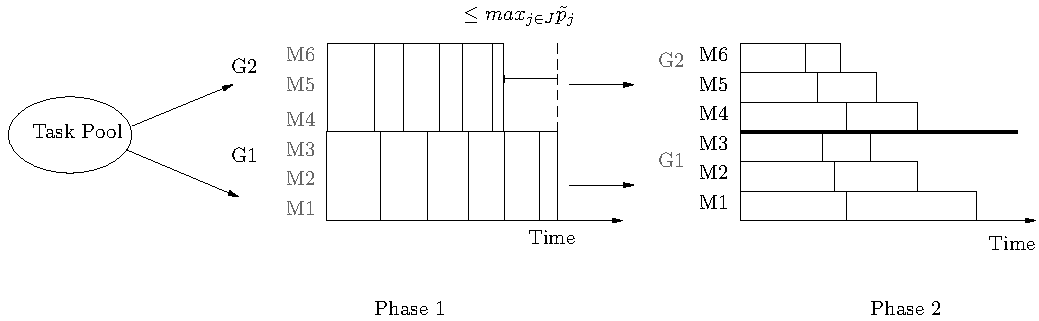
\includegraphics[width=\linewidth]{model3.pdf}
\caption{An example of replication in groups with $m = 6$, $k = 2$. In
  phase 1, the data of the tasks are assigned to one of the
  groups. Phase 2 schedules each task to a machine within the group it was 
  assigned.}
\label{fig:Model 3}
\end{figure*}

\begin{theorem}
  \label{th:strategy3}
  With $k$ groups, the competitive ratio of
  \textbf{LS-Group } is $ \frac{k\alpha^{2}}{\alpha^{2}+k-1} (1+
  {\frac{k-1}{m}} ) + \frac{m-k}{m}$
\end{theorem}
\begin{proof} 
  We assume without loss of generality that $ C_{max}$ comes from
  group $G1$. $C_{max}^{*}$ must be greater than the average of the
  loads on the machines.
  \begin{equation}{\nonumber}
    C_{max}^{*} \geq  \frac{\sum_{j \in J}^{}{{p_{j}}}}{m}
  \end{equation}

  $\sum_{j \in J }{{p_{j}}}$ can be written as sum of load on $G1$ and
  load on rest of groups.
  \begin{equation}\label{eq11}
    C_{max}^{*} \geq  \frac{\sum_{j \in G1 }^{}{{p_{j}}}+ \sum_{l=2}^{k}\sum_{j \in Gl }^{}{{p_{j}}}}{m}
  \end{equation}

  As in phase 1 tasks are allocated to different groups using List
  Scheduling with the estimated processing times of the tasks, the
  (estimated) load difference between any two groups cannot be greater
  than the estimated value of largest task ${max_{j \in J}}{\tilde
    p_{j}}$.  So, for any group $Gl \neq G1$, We have
  \begin{equation}{\nonumber}
\forall l \in \{2, 3, \dots ,k\}, \left |\sum_{j \in G1 }^{}{\tilde p_{j}}- \sum_{j \in Gl }^{}{\tilde p_{j}} \right | \leq {max_{j \in J}}{\tilde p_{j}}
  \end{equation}  
  Adding for all values of $l$ leads to
  \begin{equation}{\nonumber}
    \left | (k-1)\sum_{j \in G1 }^{}{\tilde p_{j}}- \sum_{l=2}^{k}\sum_{j \in Gl }^{}{\tilde p_{j}} \right | \leq (k-1) {max_{j \in J}}{\tilde p_{j}}
  \end{equation}

  \textbf{Case 1:} If $(k-1)\sum_{j \in G1 }^{}{\tilde p_{j}} >
  \sum_{l=2}^{k}\sum_{j \in Gl }^{}{\tilde p_{j}}$.
  \begin{equation}{\nonumber}
    \sum_{l=2}^{k}\sum_{j \in Gl }^{}{\tilde p_{j}} \geq (k-1) \left( \sum_{j \in G1 }^{}{\tilde p_{j}}- {max_{j \in J}}{\tilde p_{j}} \right)
  \end{equation}

  As the actual processing time of the tasks can vary within a factor
  $\alpha$ and $\frac{1}{\alpha}$ of their estimated processing times,
  the following inequality holds
  \begin{equation}{\nonumber}
    \alpha\sum_{l=2}^{k}\sum_{j \in Gl }^{}{{p_{j}}} \geq (k-1) \left( \frac{1}{\alpha}\sum_{j \in G1 }^{}{{p_{j}}}- \alpha {max_{j \in J}}{{p_{j}}} \right)
  \end{equation}
  \begin{equation}\label{eq9}
    \sum_{l=2}^{k}\sum_{j \in Gl }^{}{{p_{j}}} \geq (k-1) \left(\frac{1}{\alpha^{2}}\sum_{j \in G1 }^{}{{p_{j}}}-  {max_{j \in J}}{{p_{j}}} \right)
  \end{equation}

  Phase 2 applies List Scheduling in the online mode. We assumed that
  $C_{max}$ comes from $G1$. Using the guarantees of List Scheduling
  we can write,
  \begin{equation}\label{eq10}
    C_{max} \leq \frac{\sum_{j \in G1 }^{}{{p_{j}}}}{m/k} + {\frac{m/k-1}{m/k}} p_{max}
  \end{equation}
  where $p_{max}$ is actual processing time of longest task in $G1$.

  From Equation~\ref{eq9} and~\ref{eq11}, we derive
  \begin{equation}{\nonumber}
    C_{max}^{*} \geq  \frac{\sum_{j \in G1 }^{}{{p_{j}}}+ (k-1)\left(\frac{1}{\alpha^{2}}\sum_{j \in G1 }^{}{{p_{j}}}-  {max_{j \in J}}{{p_{j}}}\right)}{m}
  \end{equation}
  \begin{equation}{\nonumber}
    \alpha^{2} (mC_{max}^{*} + (k-1){max_{j \in J}}{{p_{j}}}) \geq  (\alpha^{2} + k-1) \sum_{j \in G1 }^{}{{p_{j}}}  
  \end{equation}
  \begin{equation}\label{eq12}
    \frac{\alpha^{2}}{\alpha^{2}+k-1}\left(m C_{max}^{*}+(k-1) {max_{j \in J}}{{p_{j}}}\right) \geq \sum_{j \in G1 }^{}{{p_{j}}}  
  \end{equation}
  
  Using \ref{eq10} and \ref{eq12}, We have
  \begin{align}{\nonumber}
    C_{max} \leq \frac{k\alpha^{2}}{\alpha^{2}+k-1}\left( C_{max}^{*}+\frac{k-1}{m} {max_{j \in J}}{{p_{j}}}\right)\\
    + {\frac{m/k-1}{m/k}} p_{max} \nonumber
  \end{align}
  
  As $C_{max}^{*}\geq {{max_{j \in J}}{p_{j}}}\geq p_{max}$, we have
  \begin{align}{\nonumber}
    C_{max} \leq \frac{k\alpha^{2}}{\alpha^{2}+k-1}\left( C_{max}^{*}+ {\frac{k-1}{m}}{C_{max}^{*}}\right)\\
    + {\frac{m-k}{m}} C_{max}^{*} \nonumber
  \end{align}    
  
  So, in case 1 the algorithm has a competitive ratio of,
  \begin{equation}{\nonumber}
    \frac{C_{max}}{C_{max}^{*}} \leq \frac{k\alpha^{2}}{\alpha^{2}+k-1}\left( 1+ {\frac{k-1}{m}} \right) + {\frac{m-k}{m}} \end{equation}\\
  
  \textbf{Case 2:} If $(k-1)\sum_{j \in G1 }^{}{\tilde p_{j}} \leq \sum_{l=2}^{k}\sum_{j \in Gl }^{}{\tilde p_{j}}$. \\
  
  Since the processing times of the tasks can vary within a factor
  $\alpha$ and $\frac{1}{\alpha}$ of their estimated values, the
  expression for case 2 can be written as
  \begin{equation}{\nonumber}
    \sum_{l=2}^{k}\sum_{j \in Gl }^{}{ p_{j}} \geq \frac{1}{\alpha^2} (k-1)\sum_{j \in G1 }^{}{ p_{j}}
  \end{equation}
  
  Putting this value in Equation~\ref{eq11}, we have
  \begin{equation}\label{eq13}
    C_{max}^{*} \geq \frac{\alpha^2+k-1}{m\alpha^2}\sum_{j \in G1 }^{}{ p_{j}}
  \end{equation}
  Using Equations~\ref{eq10} and~\ref{eq13}, and as $C_{max}^{*} \geq p_{max}$, we have
  \begin{equation}{\nonumber}
    C_{max} \leq \frac{k\alpha^2}{\alpha^2+k-1}C_{max}^{*}+\frac{m-k}{m}C_{max}^{*}
  \end{equation}
  
  So, in case 2 the algorithm has a competitive ratio of
  $\frac{k\alpha^2}{\alpha^2+k-1}+\frac{m-k}{m}$.

  Clearly, the algorithm has a worst competitive ratio in case 1.  So,
  the algorithm has a competitive approximation ratio of
  $\frac{C_{max}}{C_{max}^{*}} \leq \frac{k\alpha^{2}}{\alpha^{2}+k-1}
  \left( 1+ {\frac{k-1}{m}} \right) + {\frac{m-k}{m}}$.
\end{proof}

% \begin{corollary}
%   When there are $2$  groups, the competitive ratio is $ 1+
%   \frac{2}{1+\alpha^{2}} (\alpha^2-\frac{1}{m})$.
% \end{corollary}

\textbf{LS-Group} uses List Scheduling in both its phases. A LPT-based
algorithm may have better guarantee. But without performing any
replication, {\em i.e.} when $k=m$, the \textbf{LS-Group} algorithm
has a competitive ratio almost equals to \textbf{LPT-No choice}'s when
the number of machines $m$ is large and the value of $\alpha$ is
within practical range. This indicates an LPT-based algorithm for
strategy 3 would likely not have a much more interesting guarantee.

\subsection{Summarizing the Replication Bound Model}\label{sec7}
Table~\ref{tab:template} summarizes the results of this paper in terms
of approximation ratios. Based on adversary technique,
Theorem~\ref{th:model1-lb} states that there is no algorithm which can
give performance better than $\frac{\alpha^{2}m }{\alpha^{2} + m-1}$ for the model where no
replication is allowed. {\bf LPT-No Choice} is a
$\frac{2\alpha^{2}m}{2\alpha^{2}+ m-1}$-approximation that uses that
strategy. For the second strategy that replicates the data of all
tasks everywhere ( $|M_j| = |M|$), {\bf LPT-No Restriction} achieves a
competitive ratio of $1 + (\frac{m-1}{m})\frac{\alpha^{2}}{2}$.  The
third strategy uses replication within $k$ groups of size $m/k$ ({\em
  i.e.}, $|M_j| = m/k$). Using this strategy, the {\bf LS-Group}
algorithm has a competitive ratio of
$\frac{k\alpha^{2}}{\alpha^{2}+k-1}\left( 1+ {\frac{k-1}{m}} \right) +
{\frac{m-k}{m}}$.



\begin{table}[ht]
  \centering
  \begin{tabular}{|l|c|c|c|c|c|}
    \hline
    Replication & Approximation ratio  \\
    \hline
    $|M_j|=1$ & $\frac{C_{max}}{C_{max}^{*}}\leq \frac{2\alpha^{2}m}{2\alpha^{2}+ m-1}$ (Th.~\ref{th:strat1-ub})  \\
    & No approximation better than $\frac{\alpha^{2}m }{\alpha^{2} + m-1}$ (Th.~\ref{th:model1-lb})   \\
    
    \hline
    $|M_j|=m$ & $\frac{C_{max}}{C_{max}^{*}} \leq 1 + (\frac{m-1}{m})\frac{\alpha^{2}}{2}$ (Th.~\ref{th:strategy2})  \\
    & $\frac{C_{max}}{C_{max}^{*}} \leq 2-\frac{1}{m}$ \cite{Graham66}   \\
    \hline
    
    $|M_j|= \frac{m}{k} $ & $\frac{C_{max}}{C_{max}^{*}} \leq \frac{k\alpha^{2}}{\alpha^{2}+k-1} \left(1+ {\frac{k-1}{m}} \right)+ {\frac{m-k}{m}}$ (Th.~\ref{th:strategy3})  \\
%    & $\frac{C_{max}}{C_{max}^{*}} \leq  1+ \frac{2}{1+\alpha^{2}} \left(\alpha^2-\frac{1}{m}\right)$ when $k=2$ [Col. 3.1]   \\
    
    \hline
  \end{tabular}
  \caption{Summary of the contribution of this paper.
    Three proposed algorithms have guaranteed performance.
    One lower bound on approximability has been established.}
  \label{tab:template}
\end{table}


Of course, there is an inherent tradeoff between replicating data and
obtaining good values for the makespan. To better understand the
tradeoff we show in Figure~\ref{fig:Graph} how the expressions of the
guarantees (or impossibility) translate to actual values in an
approximation ratio / replication space.  We picked 3 values of
$\alpha$ while keeping the number of machines fixed to $m=210$. 

When $\alpha=1.1$, even with multiple groups {\bf LS-Group} provides little
improvement over {\bf LPT-No Choice} in terms of makespan guarantee. However there is a significant
gap between the guarantee of {\bf LPT-No Choice} and the lower bound
on possible approximation. When $\alpha$ is small, there is a
significant improvement in using {\bf LPT-No Restriction} over using
 {\bf LS-Group} with only 1 group.

When $\alpha$ increases to $1.5$, there is no more differences in the
guarantees of {\bf LS-Group} with 1 group and {\bf LPT-No
  Restriction}. Also {\bf LS-Group} provides many interesting intermediate
solutions between deploying the data on a single machine and deploying
them everywhere.

When $\alpha=2$, the range of the approximation ratios widens and
the value of the lower bound increases. Now {\bf LS-Group} is able to
get a better approximation using less than $50$ replications than 
can be guaranteed by deploying data on a single machine. Also, the
approximation ratio quickly improves from more than $7.5$ with the
data being replicated on $1$ machine to a ratio of less than $6$ with
only replicating the data on $3$ machines.

Overall, when $\alpha$ is large, only few replication improve the
performance significantly.


\begin {figure}
  \centering
  \begin{subfigure}[b]{0.5\textwidth}
    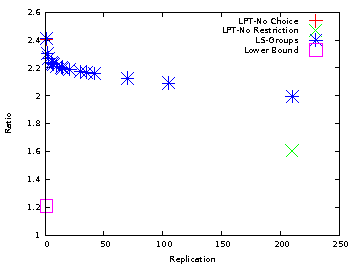
\includegraphics[width=\textwidth]{alpha_11.pdf}
    \caption{$m=210$, $\alpha=1.1$}
    \label{fig:1}
  \end {subfigure} %
  
  \begin{subfigure}[b]{0.5\textwidth}
    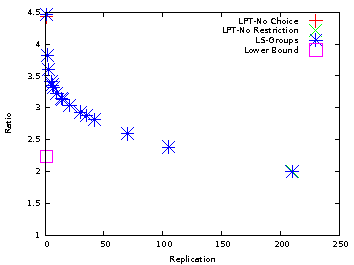
\includegraphics[width=\textwidth]{alpha_15.pdf}
    \caption{$m=210$, $\alpha=1.5$}
    \label{fig:2}
  \end {subfigure} %
  
  \begin{subfigure}[b]{0.5\textwidth}
    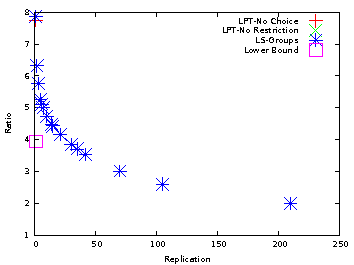
\includegraphics[width=\textwidth]{alpha_2.pdf}
    \caption{$m=210$, $\alpha=2$}
    \label{fig:3}
  \end{subfigure} %

  \caption{Ratio-Replication graph with $m=210$ and $\alpha \in \{1.1, 1.5, 2\}$.}
  \label{fig:Graph}
\end{figure}


\section{Memory Aware Replications}\label{ch5}
   
\todo{Be carfeul of $M_{max}$ and $M_j$}
   
Replication improves performance but incurs a cost in terms of memory
consumption.  Replication allows to obtain a better load balancing by
reducing the effect of uncertainties in processing times of tasks. But
each replica occupies memory, and increases the memory consumption.
So, replicating all the tasks is not possible in real scenarios. This
justify the need for an efficient replication strategy which allows an
algorithm to choose which tasks are to be replicated and where.  In
this chapter we investigate the bi-objective problem of minimizing the
makespan as well as the memory consumption. A memory-aware replication
strategy improves execution times with little increase in memory
consumption.
   
The problem is to schedule a set $J$ of $n$ tasks on $m$ machines such
that both makespan $C_{max}$ as well as memory usage $M_{max}$ is
optimized.  Let $\pi_1$ be the schedule which minimizes makespan and
$\pi_2$ be the memory-aware schedule. $\tilde{C}^{\pi_1}_{max}$ and
$\tilde{C}^{*}_{max}$ are makespan and optimal makespan when all the
tasks are scheduled according to $\pi_1$. Similarly, $M^{\pi_2}_{max}$
is memory consumption of the most occupied machine and $M^*_{max}$ is
its optimal value. The strategy is to divide tasks into two sets $S_1$
and $S_2$ such that set $S_1$ contains the processing time intensive
tasks and set $S_2$ contains the memory intensive tasks, and schedule
them differently and in such a way that it optimizes both the
objectives.
     
We propose two algorithms $SABO_\triangle$ (stands for static
asymmetric bi-objective) and $ABO_\triangle$ (stands for asymmetric
bi-objective), which are based on $SBO_\triangle$
algorithm. $SBO_\triangle$~\cite{10.1109/IPDPS.2008.4536292} is
bi-objective algorithm for minimizing makespan and memory usage for
independent tasks by combining results of two symmetric schedules each
dedicated to a single objective.
 
\subsection{The $SABO_\triangle$ Algorithm}
                     
We propose $SABO_\triangle$ Algorithm which is static in nature and
restrict each task to be scheduled to only one machine. Similar to
$SBO_\triangle$ this algorithm assigns tasks to all the machines in
phase 1 such that it minimizes both the objectives. As each task is
restricted to only one machine, there is no task replication. Based on
similar condition as in $SBO_\triangle$, a processing-time intensive
task is assigned to $\pi_1$ schedule and a memory intensive task is
assigned to $\pi_2$
                     
In phase 2, the algorithm loads the tasks to the machines they were assigned in phase 1.\\
                     
\begin{figure*}[htp]
  \centering
  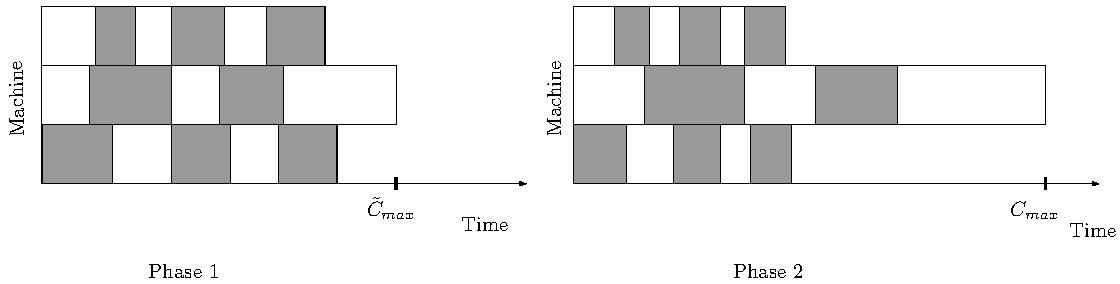
\includegraphics[width= 16 cm]{mem2.pdf}
  \caption{An example of two phases of the schedule generated by the
    $SABO_\triangle$. The uncolored parts represent tasks scheduled
    according $\pi_2$. The colored parts represents tasks scheduled
    according $\pi_1$}
  \label{fig:ch5-1}
\end{figure*} 

\begin{algorithm}                    
  \caption{$SABO_\triangle$}
  \label{alg2}
  \begin{algorithmic} 
    \State \textbf{Input:} $m$ machines 
    \State \hspace*{15pt}Set $J$ of $n$ tasks
    \State\hspace*{15pt}Let $\pi_1$ be a $ \rho_1$-approximated schedule on makespan $\tilde{C}_{max}$ 
    \State \hspace*{15pt}Let $\pi_2$ be a $\rho_2$- approximated schedule on memory ${M_{max}}$
    \State
    \State \textbf{Phase 1:} [Uses $SBO_\triangle$]
    \ForAll{$j\in J$}
    \If{$\frac{\tilde{p_j}}{\tilde{C}^{\pi_1}_{max}} \leq \triangle \frac{s_j}{M^{\pi_2}_{max}}$}
    \State Assign $j$ to a machine according to $\pi_2$ schedule
    \State Add $j$ to $S_2$
    \Else
    \State Assign $j$ to a machine according to $\pi_1$ schedule
    \State Add $j$ to $S_1$   
    \EndIf 
    \EndFor
    
    \State \textbf{End of Phase 1} 
    \State 
    \State \textbf{Phase 2:} 
    \State \hspace*{42pt}Schedule tasks to machines to which they were assigned during phase 1
    
    \State \textbf{End of Phase 2} 
    
  \end{algorithmic}
\end{algorithm}     



\begin{theorem}
  \label{th:chapter5-2a}
  The $SABO_\triangle$ Algorithm generates a $(1+\triangle)\alpha^2
  \rho_1$ - approximated schedule on makespan.
\end{theorem}         

\begin{proof}
  Let $k$ be the machine reaching the makespan $C_{max}$ of the
  schedule. $C_{max}$ can be written as the sum of processing times of
  tasks in set $S_1$ and $S_2$ scheduled on machine $k$.
  \begin{equation}\nonumber
    C_{max}= \sum_{j \in S_1 \cap E_k}^{}p_j+\sum_{j \in S_2 \cap E_k}^{}p_j 
  \end{equation}
  
  Since, $\sum\limits
  _{j \in S_2 \cap E_k}^{}p_j\leq\alpha\sum\limits
  _{j \in S_2 \cap E_k} \tilde{p}_j$
  \begin{equation}\nonumber
    C_{max} \leq \sum_{j \in S_1 \cap E_k}^{}p_j+\alpha\sum_{j \in S_2 \cap E_k} \tilde{p}_j 
  \end{equation}
  
  
  Let $C^{\pi_1}_{max}$ denotes the makespan obtained after phase 2
  when tasks are loaded and actual processing time of a task is known
  to scheduler. Since $C^{\pi_1}_{max} \geq \sum\limits _{j \in S_1
    \cap E_k}^{}p_j$ and $\sum\limits _{j \in S_2\cap E_k}\triangle
  {\tilde{C}^{\pi_1}_{max}} \frac{s_j}{M^{\pi_2}_{max}}\geq
  \sum\limits _{j \in S_2\cap E_k}^{}\tilde{p}_j $ by definition of
  $S_2$, we have
          
  \begin{equation}\nonumber
    C_{max}\leq C^{\pi_1}_{max}+\alpha\sum_{j \in S_2\cap E_k}^{}\triangle {\tilde{C}^{\pi_1}_{max}} \frac{s_j}{M^{\pi_2}_{max}}
  \end{equation}                    
  Since, $C^{\pi_1}_{max}\leq\alpha\tilde{C}^{\pi_1}_{max}$ and
  $\sum\limits_{j \in S_2\cap E_k} \frac{s_j}{M^{\pi_2}_{max}}\leq 1$,
  we have
  \begin{equation}
    \nonumber C_{max}\leq(1+\triangle)\alpha\tilde{C}^{\pi_1}_{max}
  \end{equation}
  
  Since $ \tilde{C}^{\pi_1}_{max} \leq \rho_1 \tilde{C}^{*}_{max}\leq
  \alpha\rho_1 {C}^{*}_{max}$ the algorithm has an approximation ratio
  of $(1+\triangle)\alpha^2 \rho_1$ on makespan.
\end{proof}
\begin{theorem} \label{th:chapter5-2b} The $SABO_\triangle$ Algorithm
  generates $ (1+\frac{1}{\triangle})\rho_2 $- approximated schedule
  on memory
\end{theorem}                      

\begin{proof}  
  The proof is identical to $SBO_\triangle$ algorithm and is presented
  in chapter~\ref{ch3}.
\end{proof}    
    
\subsection{The $ABO_\triangle$ Algorithm} 

We propose a two phase algorithm. In phase 1 the algorithm assigns
tasks to all the machines such that it minimizes both the makespan as
well as memory consumption. The tasks having more memory value in
comparison to its processing time are scheduled using memory intensive
schedule which aim at minimizing memory.  Similarly tasks which incur
more processing time cost compared to memory cost are assigned to
machines according to the makespan intensive schedule. These tasks are
replicated to all machines in order to provide better load balancing
and hence minimized makespan. The algorithm in its phase 1 assigns all
the memory intensive tasks to machines first, then chooses tasks
having more processing time values compared to memory they consume.
    
In phase 2, the algorithm loads the memory intensive tasks to the
machines they were assigned in phase 1 respecting the tasks assignment
during phase 1. The algorithm schedule the time intensive tasks
(replicated tasks) using Graham's List Scheduling after all the memory
intensive tasks are scheduled. Figure~\ref{fig:ch5-2} shows a schedule
instance using the algorithm.
    
\begin{figure*}[htp]
  \centering
  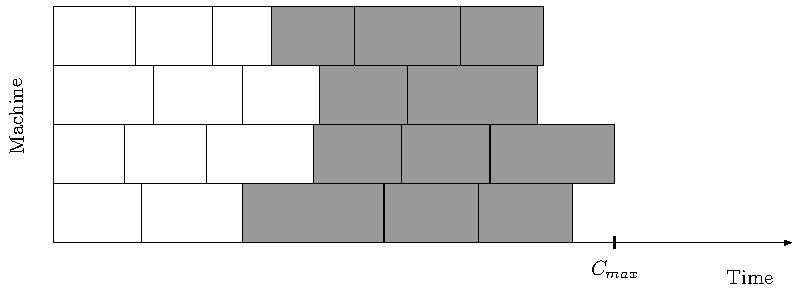
\includegraphics[width= 16 cm]{mem.pdf}
  \caption{An example of the schedule generated by the $ABO_\triangle$
    algorithm. The uncolored parts represent the memory intensive
    tasks scheduled according $\pi_2$. The colored parts represent the
    processing time intensive tasks and scheduled using LS after
    replicated}
  \label{fig:ch5-2}
\end{figure*}

\begin{algorithm}
  \caption{$ABO_\triangle$}
  \label{alg1}
  \begin{algorithmic} 
    \State \textbf{Input:} $m$ machines 
    \State \hspace*{42pt}Set $J$ of $n$ tasks
    \State\hspace*{42pt}Let $\pi_1$ be a $ \rho_1$-approximated schedule on makespan $\tilde{C}_{max}$ 
    \State \hspace*{42pt}Let $\pi_2$ be a $\rho_2$- approximated schedule on memory ${M_{max}}$
    \State
    \State \textbf{Phase 1:}
    \ForAll{$j\in J$}
    \If{$\frac{\tilde{p_j}}{\tilde{C}^{\pi_1}_{max}} \leq \triangle \frac{s_j}{M^{\pi_2}_{max}}$}
    \State Assign $j$ to a machine according to $\pi_2$ schedule
    \State Add task $j$ to set $S_2$   
    \EndIf 
    \EndFor
    \ForAll{$j\in J$}
    \If{$\frac{\tilde{p_j}}{\tilde{C}^{\pi_1}_{max}} \geq \triangle \frac{s_j}{M^{\pi_2}_{max}}$}
    \State Add $j$ to set $S_1$
    \State Replicate $j$ everywhere   
    \EndIf 
    \EndFor
    \State \textbf{End of Phase 1} 
    \State 
    \State \textbf{Phase 2:} 
    \State \hspace*{42pt}Schedule tasks from set $S_2$ respecting job assignment during phase 1
    \State \hspace*{42pt} Schedule all replicated tasks from set $S_1$ using Graham's LS Algorithm 
    \State \textbf{End of Phase 2} 
    
  \end{algorithmic}
\end{algorithm}

\begin{theorem}
  \label{th:chapter5-la}
  The $ABO_\triangle$ Algorithm generates a $
  (2-\frac{1}{m}+\triangle\alpha^2 \rho_1) $- approximated schedule on
  makespan.
\end{theorem}         
\begin{proof}
  Let $k$ be the machine reaching the makespan $C_{max}$ of the
  schedule. $C_{max}$ can be written as the sum of the processing
  times of tasks in sets $S_1$ and $S_2$ scheduled on machine $k$.
  \begin{equation}\nonumber
    C_{max}= \sum_{j \in S_1 \cap E_k}^{}p_j+\sum_{j \in S_2 \cap E_k}^{}p_j 
  \end{equation}
  
  Since, $\sum\limits_{j \in S_2 \cap
    E_k}^{}p_j\leq\alpha \sum \limits_{j \in S_2 \cap E_k} \tilde{p}_j$
  \begin{equation}\nonumber
    C_{max} \leq \sum_{j \in S_1 \cap E_k}^{}p_j+\alpha\sum_{j \in S_2 \cap E_k} \tilde{p}_j 
  \end{equation}
          
           
  Let $C^R_{max}$ denotes makespan obtained by scheduling the
  replicated tasks using LS. Since $C^R_{max} \geq \sum\limits_{j \in
    S_1 \cap E_k}^{}p_j$ and $\sum\limits_{j \in S_2\cap E_k}\triangle
  {\tilde{C}^{\pi_1}_{max}} \frac{s_j}{M^{\pi_2}_{max}}\geq
  \sum\limits _{j \in S_2\cap E_k}^{}\tilde{p}_j $ by definition of
  $S_2$, we have
  \begin{equation}\nonumber
    C_{max}\leq C^R_{max}+\alpha\sum_{j \in S_2\cap E_k}^{}\triangle {\tilde{C}^{\pi_1}_{max}} \frac{s_j}{M^{\pi_2}_{max}}
  \end{equation}
  Using the property of LS, the approximation ratio of the schedule
  incorporating only replicated tasks is $2-\frac{1}{m}$. So,
  $C^R_{max} \leq (2-\frac{1}{m})C^{*}_{max}$. Also, $\sum\limits
  _{j\in S_2\cap E_k}^{} \frac{s_j}{M^{\pi_2}_{max}}\leq 1$.
  \begin{equation}\nonumber
    C_{max}\leq (2-\frac{1}{m})C^{*}_{max}+\alpha\triangle {\tilde{C}^{\pi_1}_{max}} 
  \end{equation}
  Also, ${\tilde{C}^{\pi_1}_{max}} \leq \rho_1
  {\tilde{C}^{*}_{max}}$. Since $\tilde{C}^{*}_{max}$ is the optimal
  makespan obtained after phase 1 considering estimated processing
  times of the tasks, we have, $\tilde{C}^{*}_{max}\leq
  \alpha{C}^{*}_{max}$. So, ${\tilde{C}^{\pi_1}_{max}} \leq \alpha
  \rho_1{C}^{*}_{max}$. Using this, we have
  \begin{equation}\nonumber
    C_{max}\leq (2-\frac{1}{m}){{C}^{*}_{max}}+\alpha^2\triangle \rho_1 {{C}^{*}_{max}} 
  \end{equation}
  Hence, we proved that the algorithm generates a
  $(2-\frac{1}{m}+\triangle \alpha^2\rho_1) $- approximated schedule
  on makespan.
\end{proof}
\begin{theorem}
  \label{th:chapter5-lb}
  The $ABO_\triangle$ Algorithm generates a $
  (1+\frac{m}{\triangle})\rho_2 $- approximated schedule on memory.
\end{theorem}
        
\begin{proof}           
  When a task is replicated all its replica occupies space in memory
  and increase memory consumption. For $m$ replicas the total memory
  consumption is $m$ times of the replicated tasks. Similar to proof
  of previous theorem, the highest maximum memory occupied by any
  machine $k$ can be written as
  \begin{equation}\nonumber
    M_{max}= \sum_{j \in S_1\cap E_k}^{}s_j+\sum_{j \in S_2\cap E_k}^{}s_j           
  \end{equation}
  As each task in set $S_1$ is replicated over all the
  machines,$\sum\limits _{j \in S_1\cap E_k}^{}s_j =\sum\limits _{j
    \in S_1}^{}s_j$.
  \begin{equation}\nonumber
    M_{max} = \sum_{j\in S_1}^{}s_j+\sum_{j \in S_2\cap E_k}^{}s_j           
  \end{equation}    
  $\sum\limits_{j \in S_2\cap E_k}^{}s_j$ at most be equal to
  $M^{\pi_2}_{max} $ and $\sum\limits_{j\in S_1}s_j$ is bounded by
  $\sum\limits_{j \in J}^{} {M^{\pi_2}_{max}}
  \frac{\tilde{p_j}}{\triangle \tilde{C}^{\pi_1}_{max}} $ as per
  condition for $\pi_1$ scheduling, using this we have
  \begin{equation}\nonumber
    M_{max}\leq \sum_{j \in J}^{} {M^{\pi_2}_{max}} \frac{\tilde{p_j}}{\triangle \tilde{C}^{\pi_1}_{max}}+{M^{\pi_2}_{max}}
  \end{equation}
  Since $ \sum\limits_{j \in J}\tilde{p}_j \leq m\tilde{C}^{\pi_1}_{max} $, we have 
  \begin{equation}\nonumber
    M_{max}\leq   \frac{m}{\triangle}{M^{\pi_2}_{max}}+{M^{\pi_2}_{max}}
  \end{equation}
  Also,  ${M^{\pi_2}_{max}} \leq \rho_2 {M^{*}_{max}}$.  Hence, The Algorithm generate $ (1+\frac{m}{\triangle})\rho_2 $- approximated schedule on memory.
\end{proof}
                  
\subsection{Summarizing the Memory Aware Model}
Table~\ref{tab:template2} summarizes the results for $SABO_\triangle$
and $ABO_\triangle$ algorithms. $SABO_\triangle$ is similar to $
SBO_\triangle$ algorithm in its first phase and has a approximation
ratio of $[(1+\triangle)\alpha^2 \rho_1,
(1+\frac{1}{\triangle})\rho_2]$ on makespan and memory.
$ABO_\triangle$ is a $ [(2-\frac{1}{m}+\triangle\alpha^2 \rho_1),
(1+\frac{m}{\triangle})\rho_2] $-approximated algorithm on makespan
and memory and replicate processing time intensive tasks to improve
makespan.
     
\begin{table}[ht]
  \centering
  \begin{tabular}{|l|c|c|c|c|c|}
    \hline
    Algorithm & Approx. on makespan & Approx. on memory  \\
    \hline
    $SABO_\triangle$&
    $(1+\triangle)\alpha^2 \rho_1$ (Th.~\ref{th:chapter5-2a})& $(1+\frac{1}{\triangle})\rho_2$ (Th.~\ref{th:chapter5-2b})   \\
    \hline
    $ABO_\triangle$&
    $(2-\frac{1}{m}+\triangle\alpha^2 \rho_1)$ (Th.~\ref{th:chapter5-la})& $(1+\frac{m}{\triangle})\rho_2$ (Th.~\ref{th:chapter5-lb})   \\
    
    
    
    % & $\frac{C_{max}}{C_{max}^{*}} \leq  1+ \frac{2}{1+\alpha^{2}} \left(\alpha^2-\frac{1}{m}\right)$ when $k=2$ [Col. 3.1]   \\
    
    \hline
  \end{tabular}
  \caption{Summary of the results of the algorithm $SABO_\triangle$ and the algorithm $ABO_\triangle$.}
  \label{tab:template2}
\end{table}
     
     
\begin{figure}
  \centering
  \begin{subfigure}[b]{0.5\textwidth}
    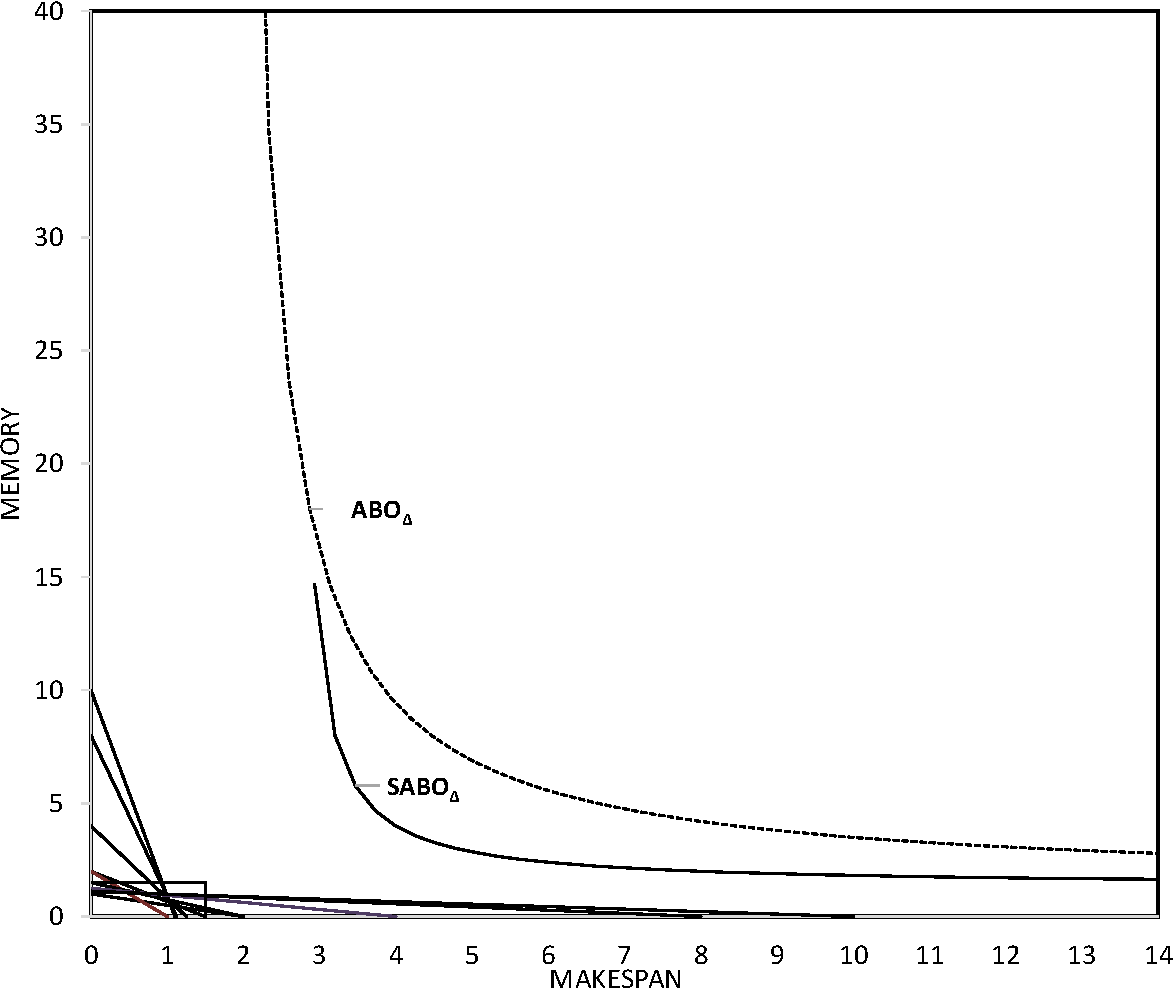
\includegraphics[width=\textwidth]{m5alpha2rho133.pdf}
    \caption{$m=5$, $\alpha^2=2$, $\rho_1=\rho_2=4/3$}
    \label{fig:ch5-3.1}
  \end {subfigure} %
  
  \begin{subfigure}[b]{0.5\textwidth}
    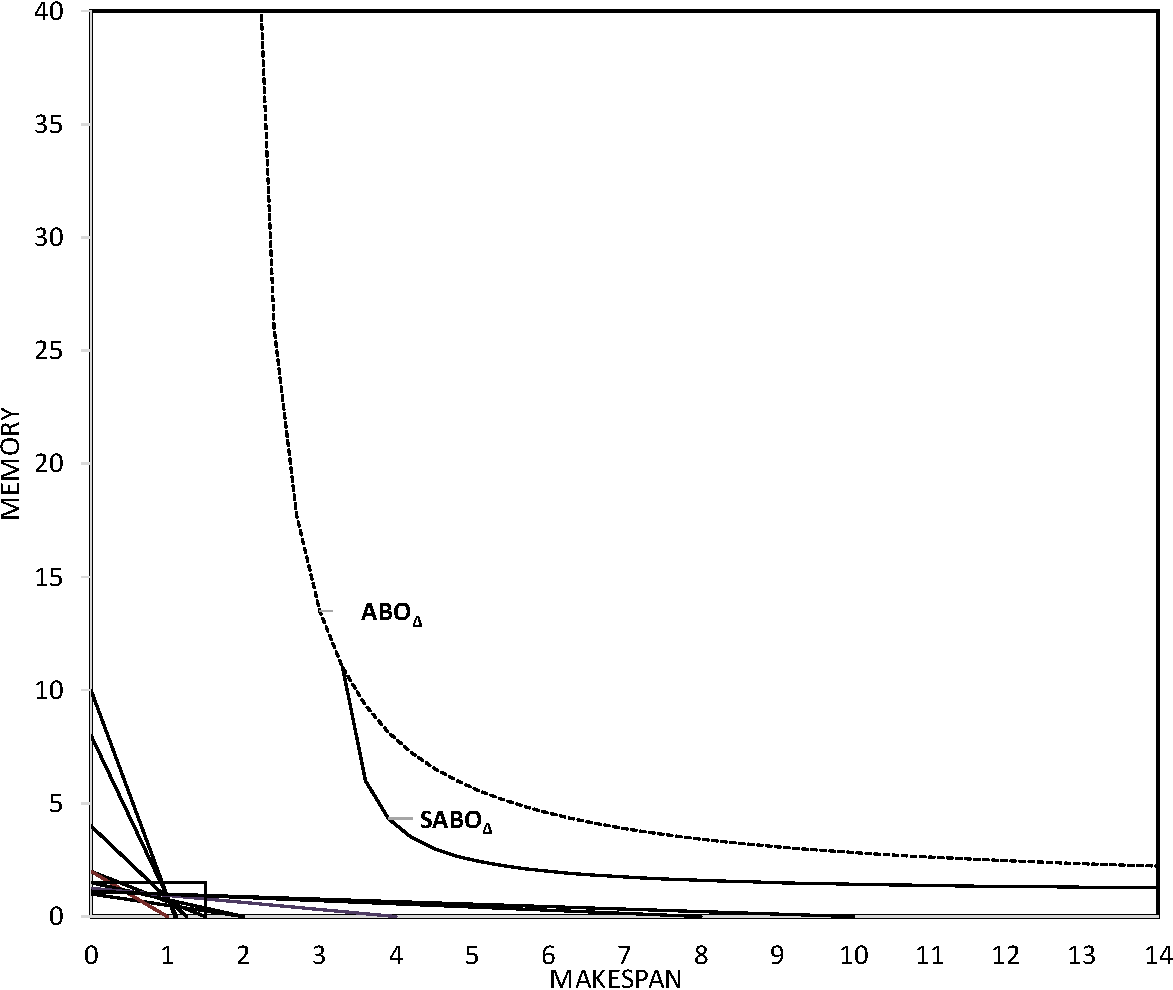
\includegraphics[width=\textwidth]{m5alpha3rho1.pdf}
    \caption{$m=5$, $\alpha^2=3$, $\rho_1=\rho_2=1$}
    \label{fig:ch5-3.2}
  \end {subfigure} %
  
  \begin{subfigure}[b]{0.5\textwidth}
    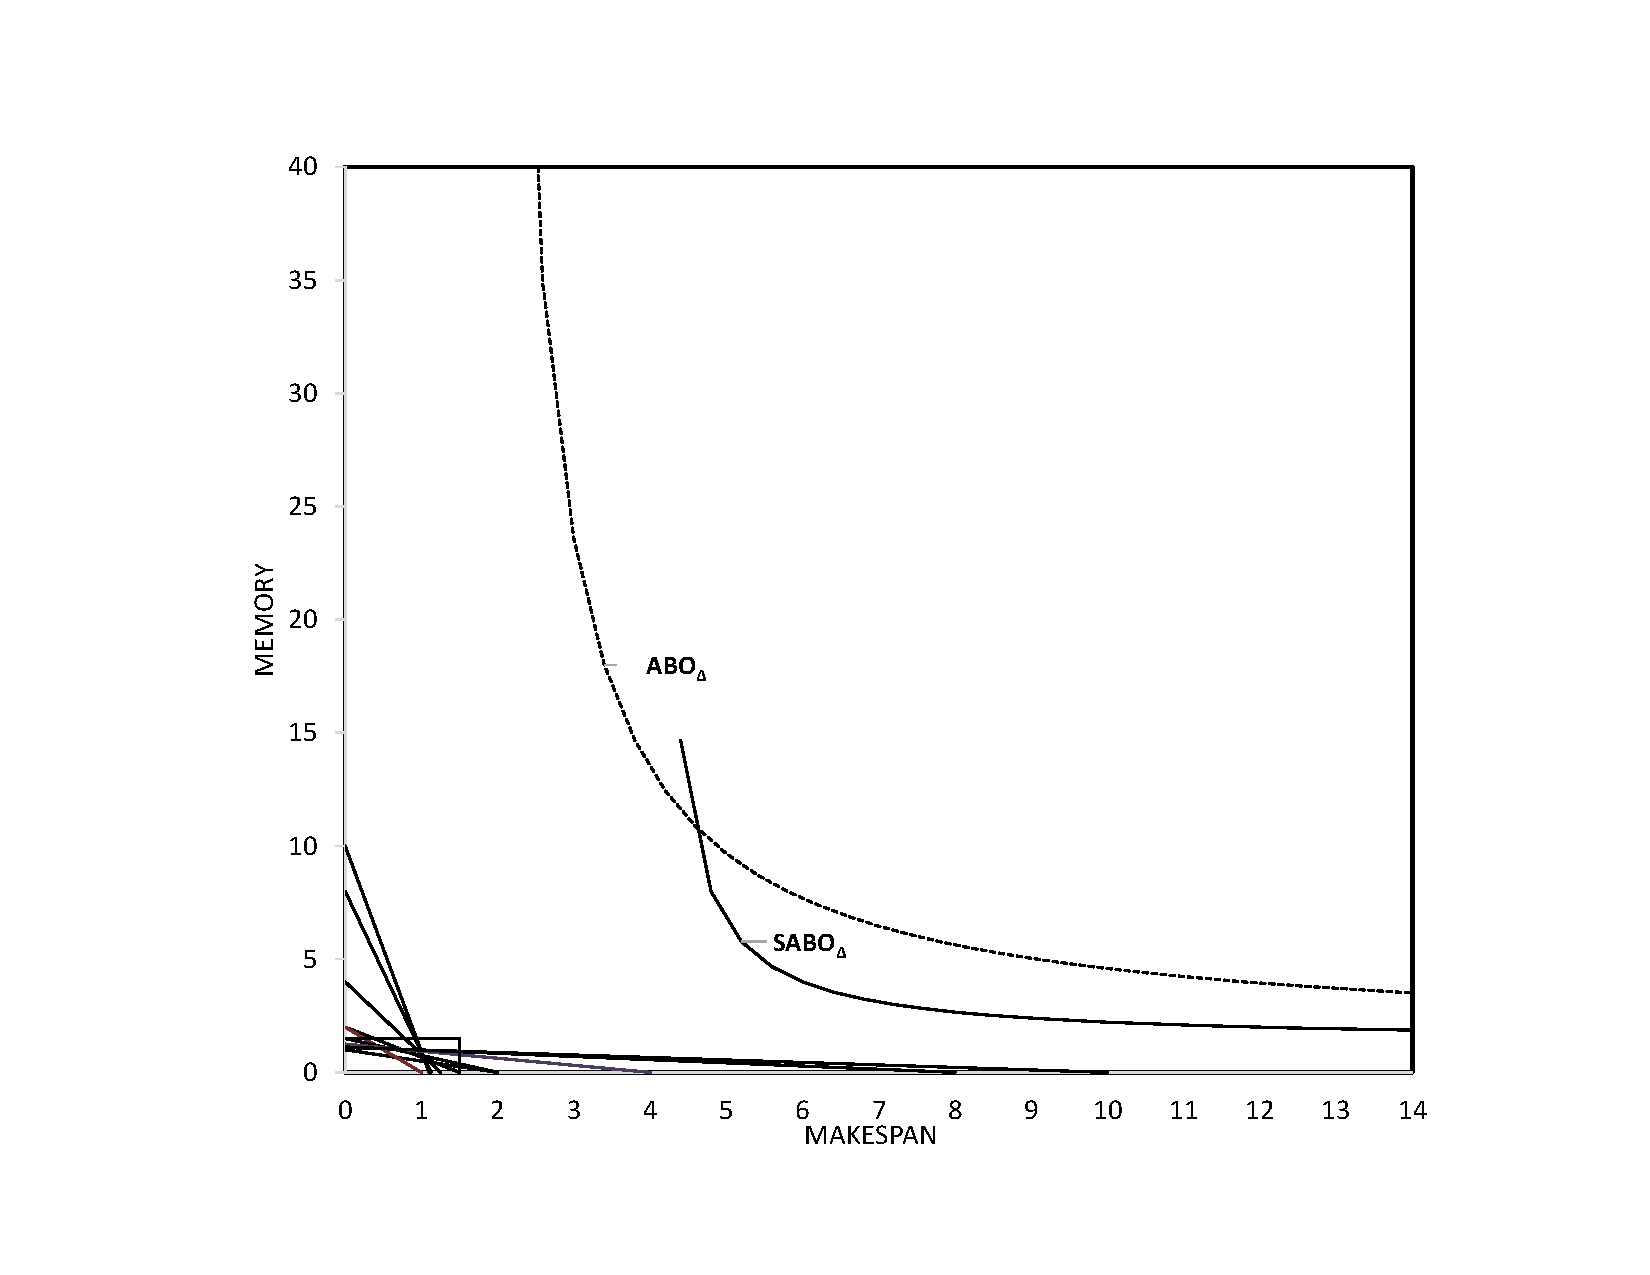
\includegraphics[width=\textwidth]{m5alpha3rho133.pdf}
    \caption{$m=5$, $\alpha^2=3$, $\rho_1=\rho_2=4/3$}
    \label{fig:ch5-3.3}
  \end{subfigure} %
  
  \caption{Memory-Makespan graph for $SABO_\triangle$ and
    $ABO_\triangle$. The bold lines represent impossibilities in
    tradeoff between guarantees.}
  \label{fig:ch5-3}
\end{figure}

To better understand the tradeoff between memory consumption and
makespan Figure~\ref{fig:ch5-3} shows memory-makespan guarantees for
the two algorithms.  The bold lines shows impossibilities in the
tradeoff between makespan and memory and means that no algorithm can
guarantee better tradeoff than this. \cite{10.1109/IPDPS.2008.4536292}
discusses about these impossibilities in context of $SBO_\triangle$
algorithm.
   
The graph shows that for higher values for $\alpha$ the algorithm
$ABO_\triangle$ have better tradeoff between memory-makespan than that
of $SABO_\triangle$. For $\alpha\rho_1\geq 2$, $ABO_\triangle$ always
have better guarantee on makespan than $SABO_\triangle$. So, a
schedule more centric to optimize makespan should follow
$ABO_\triangle$ algorithm. And a memory centric schedule should follow
$SABO_\triangle$ as the algorithm always has better guarantee on
memory.
   
As a system designer, one always want to pick the algorithm and
parameters that is best tradeoff between makespan and memory
consumption.  Depending on the guarantee, one should either pick
$ABO_\triangle$ or $SABO_\triangle$ for scheduling tasks.  For
instance, if you want to guarantee a makespan less than 3 as in the
case depicted in Figure~\ref{fig:ch5-3.2}, you should use
$ABO_\triangle$. However if you want a better guarantee on memory, you
should always use $SABO_\triangle$ for task scheduling.
     

\section{Conclusion and Future Work}\label{sec8}

We studied the effect of uncertainty in the processing time of tasks
when scheduling for parallel and distributed machines. In particular, we
investigated how allowing tasks to execute on different machines can
help dealing with not knowing the processing time of tasks
accurately. We investigated three different replication strategies,
provided an approximation algorithm in each case and a lower bound on the
best achievable approximation in one of the case. The various
strategies allow to trade the number of replication for a better
guarantee. In particular, we obtained a better guarantee with fewer
replication than can be achieved by putting the data of a task on only
one machine. We observed that even a small amount of replications can
improve the guarantee significantly. Therefore, we concluded that
deploying the data on multiple machines can be an effective way of
dealing with processing time uncertainties.

There are some open problems which can be explored further. Better
lower bounds might help understanding the problem better: clearly when
$\alpha$ is low, the problem is no different than the offline problem,
and when it is large, the problem converges to the non-clairvoyant
online problem. Having a clearer idea of where the boundary is will
certainly prove useful in understanding how much can be gained using
data replication. Also, while replicating data using groups of
machines proved effective, more general replication policies can
certainly lead to better guarantees.

Though, we assumed that every tasks were replicated the same amount of
time. A more realistic model would introduce a cost of replicating a
task (either global or per machine). This would allow to replicate
only some critical tasks and limit memory usage.

\bibliographystyle{spmpsci}
\bibliography{josh} 



\end{document}


